% Copyright (c) 2022 by Lars Spreng
% This work is licensed under the Creative Commons Attribution 4.0 International License.
% To view a copy of this license, visit http://creativecommons.org/licenses/by/4.0/ or send a letter to Creative Commons, PO Box 1866, Mountain View, CA 94042, USA.
%
%~~~~~~~~~~~~~~~~~~~~~~~~~~~~~~~~~~~~~~~~~~~~~~~~~~~~~~~~~~~~~~~~~~~~~~~~~~~~~~
% Roameo: agents plan the trip, you make the call. Seven-minute presentation (420 s at most: the
% title and ten timed slides, then backup slides). Authors: Zhen Lu and Noctis Zhang.
% Speaker notes for each slide live in the \note{...} blocks and match pres-note.md.
% Uncomment the \setbeameroption line below to see them.
%
% The story and the figures follow ../STORY_PLAN.md: assertion and evidence (a full-sentence title,
% one visual, at most two short lines). Every number comes from the repository: the evaluation
% files docs/evaluation_results(.md, .json) and docs/evaluation_results_llm(.md, .json), README.md,
% the code under backend/, and one real run of the app shown in docs/screenshots/.
% Build: latexmk -pdf slides.tex (figures first: see ../README.md).
%~~~~~~~~~~~~~~~~~~~~~~~~~~~~~~~~~~~~~~~~~~~~~~~~~~~~~~~~~~~~~~~~~~~~~~~~~~~~~~

\documentclass[
t,11pt,notheorems,usepdftitle=false,hyperref={pdfauthor={Zhen Lu and Noctis Zhang},pdftitle={Roameo: agents plan the trip, you make the call},pdfsubject={Seven-minute project presentation}}
]{beamer}
% Keep the PDF metadata to title, author and subject.
\pdfsuppressptexinfo=-1
\hypersetup{pdfcreator={},pdfproducer={}}


% Copyright (c) 2022 by Lars Spreng
% This work is licensed under the Creative Commons Attribution 4.0 International License. 
% To view a copy of this license, visit http://creativecommons.org/licenses/by/4.0/ or send a letter to Creative Commons, PO Box 1866, Mountain View, CA 94042, USA.

%~~~~~~~~~~~~~~~~~~~~~~~~~~~~~~~~~~~~~~~~~~~~~~~~~~~~~~~~~~~~~~~~~~~~~~~~~~~~~~
% Add your packages and commands to this file
%~~~~~~~~~~~~~~~~~~~~~~~~~~~~~~~~~~~~~~~~~~~~~~~~~~~~~~~~~~~~~~~~~~~~~~~~~~~~~~

%~~~~~~~~~~~~~~~~~~~~~~~~~~~~~~~~~~~~~~~~~~~~~~~~~~~~~~~~~~~~~~~~~~~~~~~~~~~~~~
% Fonts
% \RequirePackage{palatino} % for serif slides
% \usefonttheme{serif}
\RequirePackage[scaled]{helvet} % for sans-serif slides

\RequirePackage[utf8]{inputenc}
\RequirePackage[T1]{fontenc}


\usepackage{styles/elegantmacros}
\usefolder{styles}
\usetheme[style=gray]{elegant}

\newcommand{\makepart}[1]{ % For convenience
\part{#1} \frame{\partpage}
}

%~~~~~~~~~~~~~~~~~~~~~~~~~~~~~~~~~~~~~~~~~~~~~~~~~~~~~~~~~~~~~~~~~~~~~~~~~~~~~~

%~~~~~~~~~~~~~~~~~~~~~~~~~~~~~~~~~~~~~~~~~~~~~~~~~~~~~~~~~~~~~~~~~~~~~~~~~~~~~~
% Figures
\RequirePackage{booktabs}
\RequirePackage{colortbl}
\RequirePackage{ragged2e}
\RequirePackage{schemabloc}
%\RequirePackage{natbib}
\RequirePackage{caption}
\RequirePackage{subcaption}
\RequirePackage{tabularx}
\RequirePackage{array}
\RequirePackage{multirow}
% biblatex and references.bib from the template are not used by this deck.
\newcolumntype{Y}{>{\centering\arraybackslash}X}

%~~~~~~~~~~~~~~~~~~~~~~~~~~~~~~~~~~~~~~~~~~~~~~~~~~~~~~~~~~~~~~~~~~~~~~~~~~~~~~

%~~~~~~~~~~~~~~~~~~~~~~~~~~~~~~~~~~~~~~~~~~~~~~~~~~~~~~~~~~~~~~~~~~~~~~~~~~~~~~
% Figures
\RequirePackage{wrapfig}
\RequirePackage{pgfplots}
\RequirePackage{graphicx}
\RequirePackage{adjustbox}
\RequirePackage{environ}
\pgfplotsset{compat=1.18}

\makeatletter
\newsavebox{\measure@tikzpicture}
\NewEnviron{scaletikzpicturetowidth}[1]{%
  \def\tikz@width{#1}%
  \def\tikzscale{1}\begin{lrbox}{\measure@tikzpicture}%
  \BODY
  \end{lrbox}%
  \pgfmathparse{#1/\wd\measure@tikzpicture}%
  \edef\tikzscale{\pgfmathresult}%
  \BODY
}
\makeatother
%~~~~~~~~~~~~~~~~~~~~~~~~~~~~~~~~~~~~~~~~~~~~~~~~~~~~~~~~~~~~~~~~~~~~~~~~~~~~~~

%~~~~~~~~~~~~~~~~~~~~~~~~~~~~~~~~~~~~~~~~~~~~~~~~~~~~~~~~~~~~~~~~~~~~~~~~~~~~~~
% Maths 
\RequirePackage{textcomp}
\RequirePackage{amsmath} 
\RequirePackage{amsthm}
\RequirePackage{mathtools}
%\RequirePackage{bbm}
%\RequirePackage{algorithm}
%\RequirePackage[osf,sc]{mathpazo}
%\RequirePackage{pifont}
%\newcommand{\xmark}{\ding{55}}%
%\numberwithin{equation}{section}
\DeclareMathOperator*{\argmax}{arg\,max}
\DeclareMathOperator*{\argmin}{arg\,min}

\setbeamertemplate{theorems}[numbered] % to number

\theoremstyle{definition}
\newtheorem{fact}{Fact}[section]
\newtheorem{examp}{Example}[section]

\theoremstyle{plain}
\newtheorem{definition}{Definition}[section]
\newtheorem{proposition}{Proposition}
\newtheorem{theorem}{Theorem}
\newtheorem{assumption}{Assumption}

\providecommand{\H}{\mathscr{H}}      
\providecommand{\E}{\mathbb{E}}
\makeatletter
\def\munderbar#1{\underline{\sbox\tw@{$#1$}\dp\tw@\z@\box\tw@}}
\makeatother

%~~~~~~~~~~~~~~~~~~~~~~~~~~~~~~~~~~~~~~~~~~~~~~~~~~~~~~~~~~~~~~~~~~~~~~~~~~~~~~
 % Loads packages and some defined commands
\usepackage{appendixnumberbeamer} % backups are not counted in the slide total
\usepackage{fontawesome5}
\usepackage{qrcode}

% \setbeameroption{show notes} % uncomment to render speaker notes alongside slides

% The template ships \emphasize as an environment. Redefine it as a one-argument command.
\renewcommand{\emphasize}[1]{\textcolor{primary}{#1}}

\graphicspath{{figures/}{../screenshots/}}
\hyphenpenalty=10000
\exhyphenpenalty=10000

% Colours shared with figures/figstyle.tex: the app's teal is the brand, one warm accent for the
% budget gap only, green for a confirmed result.
\definecolor{primary}{HTML}{0F766E}
\definecolor{accent}{HTML}{C2410C}
\definecolor{ok}{HTML}{4D7C0F}
\definecolor{ink}{HTML}{1F1F1F}
\definecolor{muted}{HTML}{5F6368}
\definecolor{rulegrey}{HTML}{C4C4C4}
\setbeamercolor{frametitle}{fg=primary}
\setbeamercolor{normal text}{fg=ink}

% Small caption under a figure, and the one or two supporting lines of a slide.
\newcommand{\figcaption}[1]{{\scriptsize\color{muted}#1\par}}
\newcommand{\support}[1]{{\small #1\par}}
% The ticking budget: a small wallet marker in the top right corner of the story slides.
\newcommand{\budget}[2]{%
  \begin{tikzpicture}[remember picture, overlay]
    \node[anchor=north east, inner sep=0pt, font=\small\bfseries, text=#1] at ([xshift=-15mm, yshift=-5mm]current page.north east) {\faWallet\hspace{0.45em}#2};
  \end{tikzpicture}}
% A rounded option button, as in the app.
\newcommand{\option}[1]{\tikz[baseline=(b.base)]\node[draw=primary, line width=0.8pt, rounded corners=7pt, inner sep=4pt, text=ink, font=\small] (b) {#1};}

\title[Roameo]{Roameo}
\subtitle{Agents plan the trip. You make the call.}
\author[Zhen Lu and Noctis Zhang]{Zhen Lu \quad Noctis Zhang}
\date{PEAAII AI Applications Hackathon 2026, Agentic AI. October 2026}

\begin{document}
\hypersetup{pdftitle={Roameo: agents plan the trip, you make the call}}

% ~~~~~~~~~~~~~~~~~~~~~~~~~~~~~~~~~~~~~~~~~~~~~~~~~~~~~~~~~~~~~~~~~~~~~~~~~~~~~~
% 1. TITLE (13 s)
{
\setbeamertemplate{footline}{}
\begin{frame}
  \vspace{1.25cm}
  \begin{columns}[T]
    \begin{column}{0.60\textwidth}
      {\footnotesize\color{muted}PEAAII AI Applications Hackathon 2026, Agentic AI\par}
      \vspace{0.5cm}
      {\fontsize{40}{44}\selectfont\bfseries\color{primary}Roameo\par}
      \vspace{0.2cm}
      {\Large\color{ink}Agents plan the trip.\\You make the call.\par}
      \vspace{0.45cm}
      {\small An AI trip planner for \textbf{students and budget travellers}. It does the research and the math, and \textbf{asks you} before it goes over your budget.\par}
      \vspace{0.45cm}
      {\normalsize\bfseries Zhen Lu \quad Noctis Zhang\par}
      {\footnotesize\color{muted}October 2026\par}
      \vspace{0.35cm}
      
\begin{tikzpicture}[x=1cm, y=1cm]
        \node[anchor=north west, inner sep=0pt] at (0,0) {\qrcode[height=1.8cm]{https://roameo-l13h.onrender.com/}};
        \node[anchor=north west, inner sep=0pt, align=left, font=\scriptsize] at (2.0,0) {\textbf{Try it}\\roameo-l13h\\.onrender.com};
        \node[anchor=north west, inner sep=0pt] at (4.4,0) {\qrcode[height=1.8cm]{https://github.com/TinyZhen/Travel_Agent}};
        \node[anchor=north west, inner sep=0pt, align=left, font=\scriptsize] at (6.4,0) {\textbf{Code}\\github.com\\/TinyZhen\\/Travel\_Agent};
      \end{tikzpicture}
    \end{column}
    \begin{column}{0.38\textwidth}
      \vspace{0.1cm}
      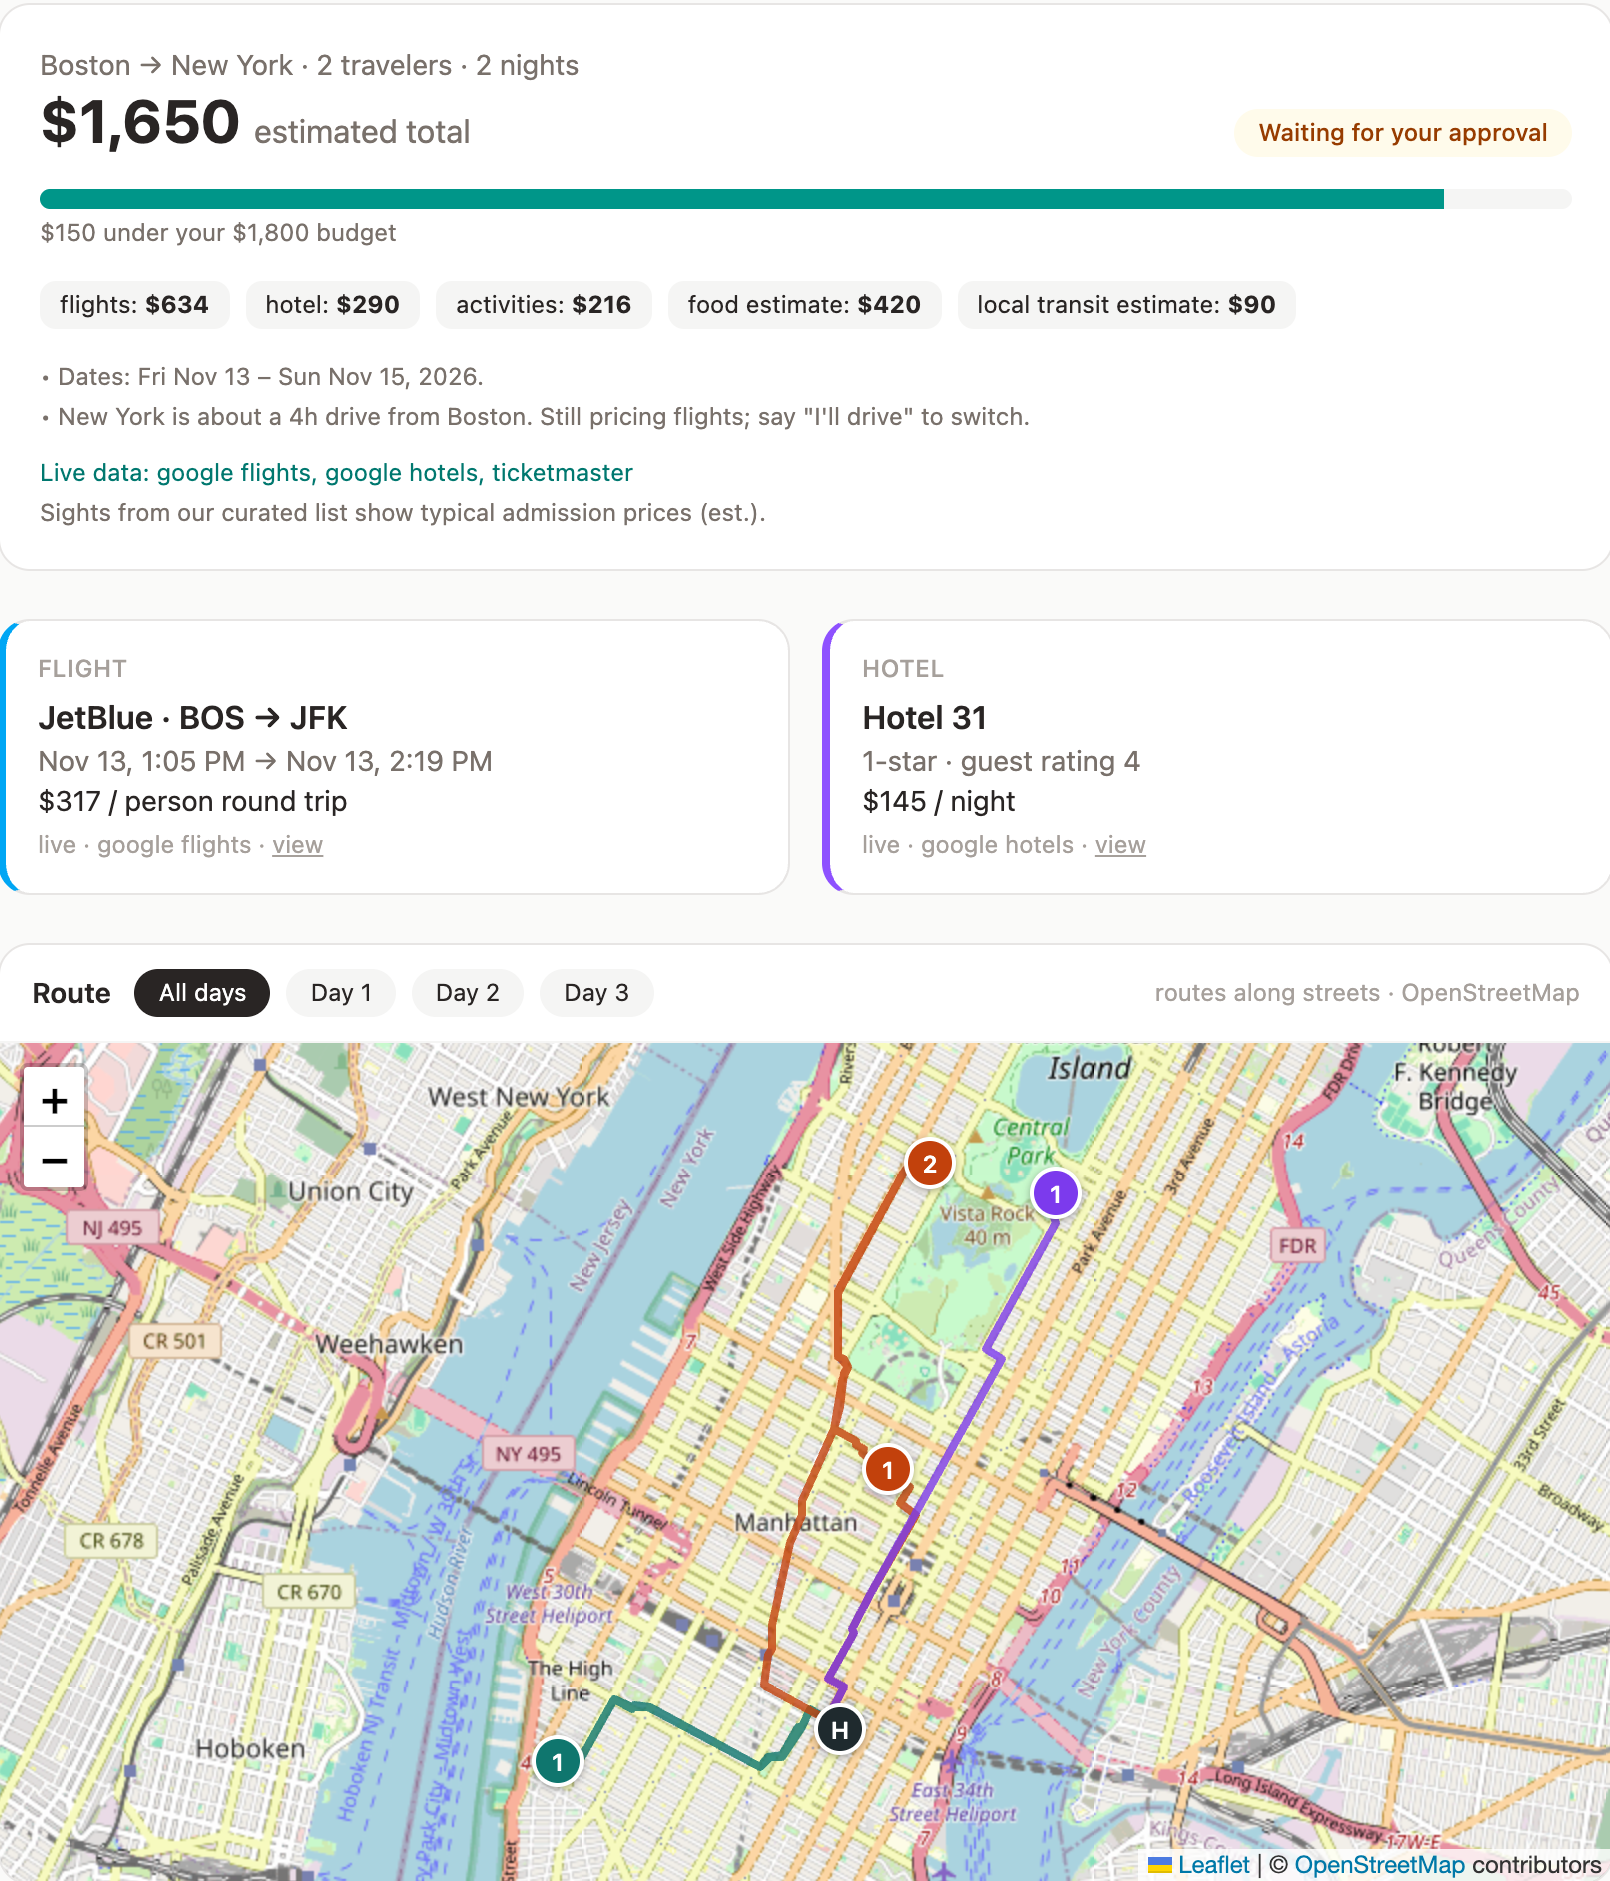
\includegraphics[width=\linewidth]{plan.png}
      \figcaption{A plan in the app: total against the budget, flight, hotel and each day's route.}
    \end{column}
  \end{columns}
  \note{
    \textbf{(13s, ends 0:13)} Hi, we are Zhen Lu and Noctis Zhang. This is Roameo, an AI trip
    planner for students and budget travellers. Its agents plan the trip, and you make the call.
  }
\end{frame}
}

% ~~~~~~~~~~~~~~~~~~~~~~~~~~~~~~~~~~~~~~~~~~~~~~~~~~~~~~~~~~~~~~~~~~~~~~~~~~~~~~
% 2. THE PERSONA AND THE CONSTRAINT (31 s)
\begin{frame}{Alex has \$600 and one sentence}
  \budget{ink}{\$600 budget}
  \vfill
  \begin{columns}[c]
    \begin{column}{0.66\textwidth}
      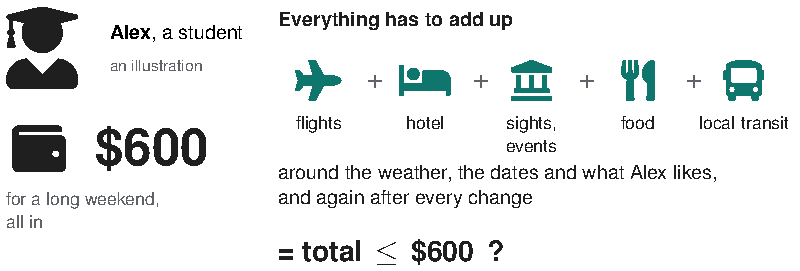
\includegraphics[width=\linewidth]{fig_persona.pdf}
    \end{column}
    \begin{column}{0.32\textwidth}
      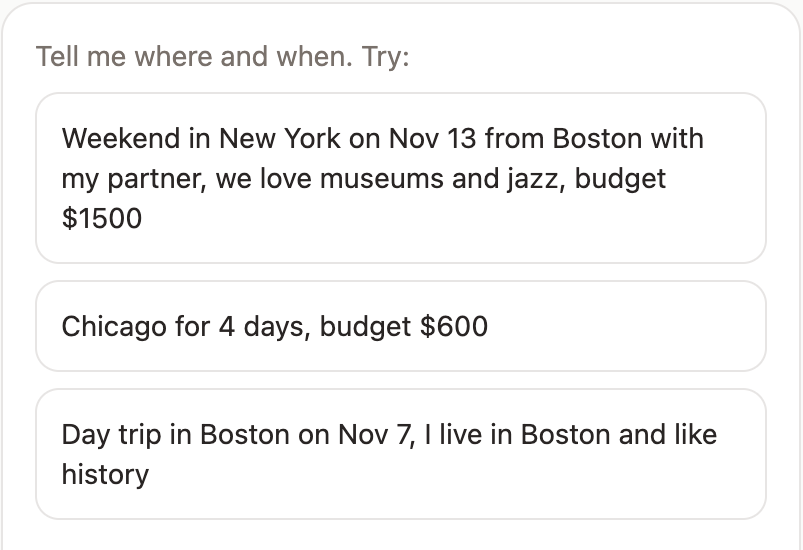
\includegraphics[width=\linewidth]{start.png}
      \figcaption{The request is the app's own example on its start screen.}
    \end{column}
  \end{columns}
  \vfill
  {\normalsize\bfseries A chat reply that adds the prices itself can say \emph{it fits your budget} with nobody checking the sum.\par}
  \vspace{0.15cm}
  \figcaption{Alex is an illustration. Booking.com's 2025 Global AI Sentiment Report, cited in our project report: 89\% of travellers want AI help planning trips, 12\% are comfortable with AI deciding alone.}
  \vspace{0.1cm}
  \note{
    \textbf{(31s, ends 0:44)} Meet Alex, a student we made up for this talk. Alex has six
    hundred dollars for a long weekend and types one sentence: Chicago for four days, budget six
    hundred dollars. Simple to say. But flights, a hotel, sights, food and transit all have to
    add up, around the weather and the dates, and again after every change. A chat reply can do
    that sum itself and say it fits, with nobody checking.
  }
\end{frame}

% ~~~~~~~~~~~~~~~~~~~~~~~~~~~~~~~~~~~~~~~~~~~~~~~~~~~~~~~~~~~~~~~~~~~~~~~~~~~~~~
% 3. THE STORY (42 s)
\begin{frame}{One sentence becomes a checked plan, and Alex keeps the final say}
  \budget{ink}{\$600 budget}
  \vspace{0.35cm}
  \begin{center}
    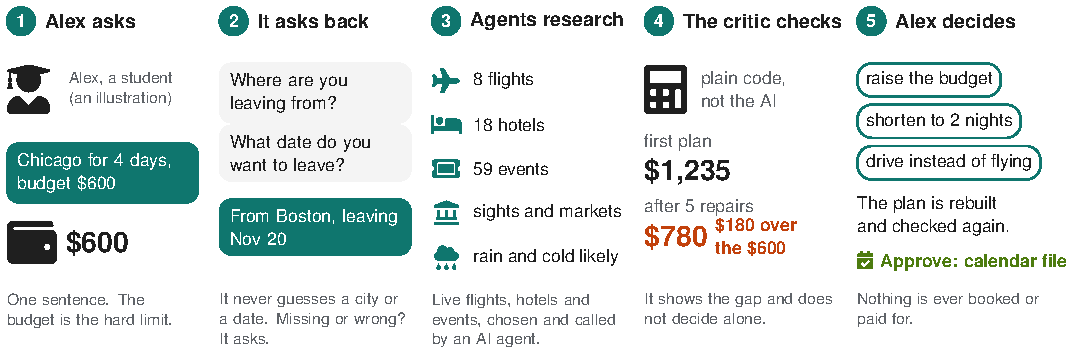
\includegraphics[width=\textwidth]{fig_story.pdf}
  \end{center}
  \vfill
  \support{An \textbf{agent} is an AI helper with one job. The \textbf{critic} is plain code that checks the cost against the budget.}
  \figcaption{Every word and number above is from one real run of the app with live flights, hotels and events (the app's screenshot of this run is on the next slides).}
  \vspace{0.15cm}
  \note{
    \textbf{(43s, ends 1:27)} Here is one real run of the app. First, Roameo asked back: where
    are you leaving from, and what date? It never guesses a city or a date. Alex answered: from
    Boston, leaving November twentieth. Then the agents went to work. An agent is an AI helper
    with one job. They found eight flights, eighteen hotels and fifty nine events, and saw rain
    and cold typical for those dates. The first plan cost one thousand two hundred thirty five
    dollars. The critic cut it to seven hundred eighty. Still one hundred eighty over. So Roameo
    did not decide. It asked Alex.
  }
\end{frame}

% ~~~~~~~~~~~~~~~~~~~~~~~~~~~~~~~~~~~~~~~~~~~~~~~~~~~~~~~~~~~~~~~~~~~~~~~~~~~~~~
% 4. THE SYSTEM (59 s)
\begin{frame}{AI agents gather, plain code checks the money, you decide twice}
  \vspace{-0.1cm}
  \begin{center}
    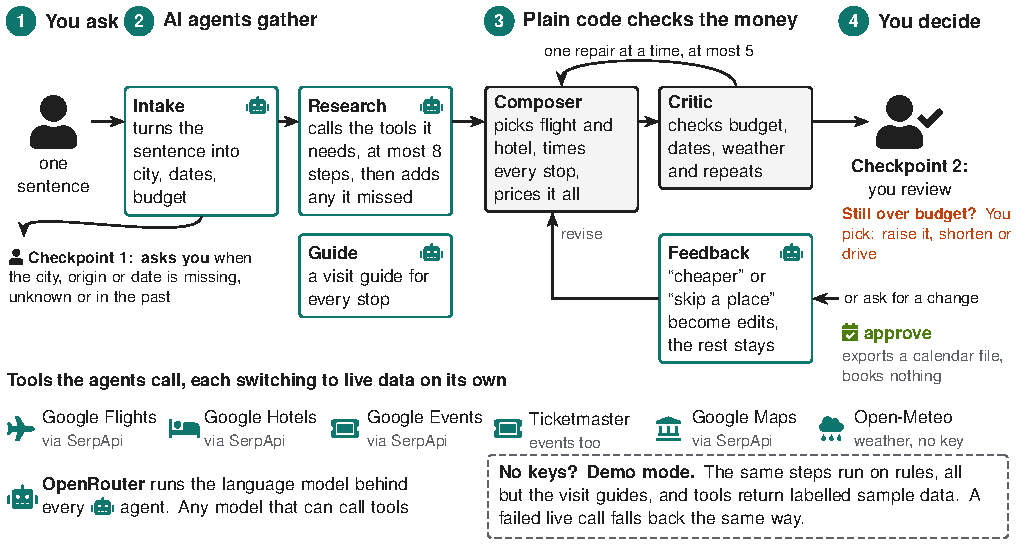
\includegraphics[height=8.55cm]{fig_system.pdf}
  \end{center}
  \note{
    \textbf{(60s, ends 2:27)} One, you ask. Two, AI agents gather. The intake agent turns your
    sentence into a city, dates and a budget. If something is missing or in the past, it asks
    you. That is the first human checkpoint. The research agent chooses which tools to call, and
    a final check adds any it skipped. Three, plain code checks the money. The composer prices
    every stop, and the critic repairs the plan one step at a time, at most five times. The AI
    never adds up the budget. Four, you decide, the second checkpoint. You approve, or ask for a
    change, and the feedback agent turns it into edits. Why agents? Each step depends on what
    the last one found. With no keys at all, demo mode runs the same steps on rules and labelled
    sample data, all but the visit guides.
  }
\end{frame}

% ~~~~~~~~~~~~~~~~~~~~~~~~~~~~~~~~~~~~~~~~~~~~~~~~~~~~~~~~~~~~~~~~~~~~~~~~~~~~~~
% 5. THE CRITIC AT WORK (41 s)
\begin{frame}{The critic re-checks each repair, and stops after five}
  \budget{accent}{\$1,235 to \$780}
  \vspace{0.1cm}
  \begin{center}
    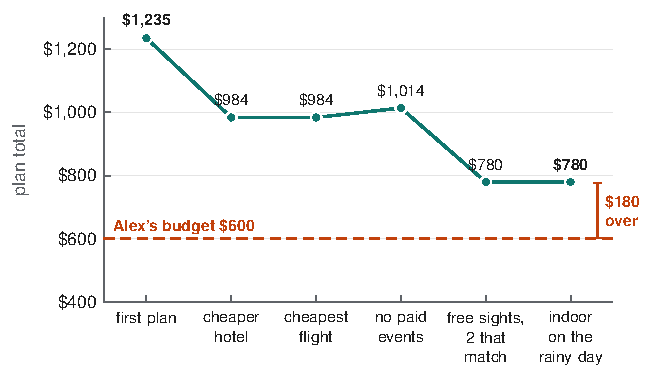
\includegraphics[height=6.3cm]{fig_critic.pdf}
  \end{center}
  \figcaption{Alex's run, read from the app's own log of what the agents did. Each point is one review by the critic, labelled with the repair just made.}
  \vfill
  \support{Each repair rebuilds the plan, so one step even went up. The limit is five repairs, then a human decides.}
  \support{In our tests a \$300 budget gets the same honest answer: \$778, which is \$478 over.}
  \vspace{0.15cm}
  \note{
    \textbf{(44s, ends 3:11)} Here is the critic in Alex's run, from the app's own log. A
    cheaper hotel took the plan from one thousand two hundred thirty five to nine hundred eighty
    four dollars. The cheapest flight did not help. Dropping paid events even went up a little,
    because each repair rebuilds the plan. Keeping free sights plus two that match Alex's
    interests reached seven hundred eighty. Moving stops indoors for the rainy day kept it
    there. Five repairs is the limit. Our tests check the same behaviour: with a three hundred
    dollar budget, it reports four hundred seventy eight over instead of hiding it.
  }
\end{frame}

% ~~~~~~~~~~~~~~~~~~~~~~~~~~~~~~~~~~~~~~~~~~~~~~~~~~~~~~~~~~~~~~~~~~~~~~~~~~~~~~
% 6. THE HUMAN DECISION (36 s)
\begin{frame}{Then it stops and asks Alex, instead of quietly going over}
  \budget{accent}{\$180 over}
  \vspace{0.1cm}
  \begin{columns}[T]
    \begin{column}{0.60\textwidth}
      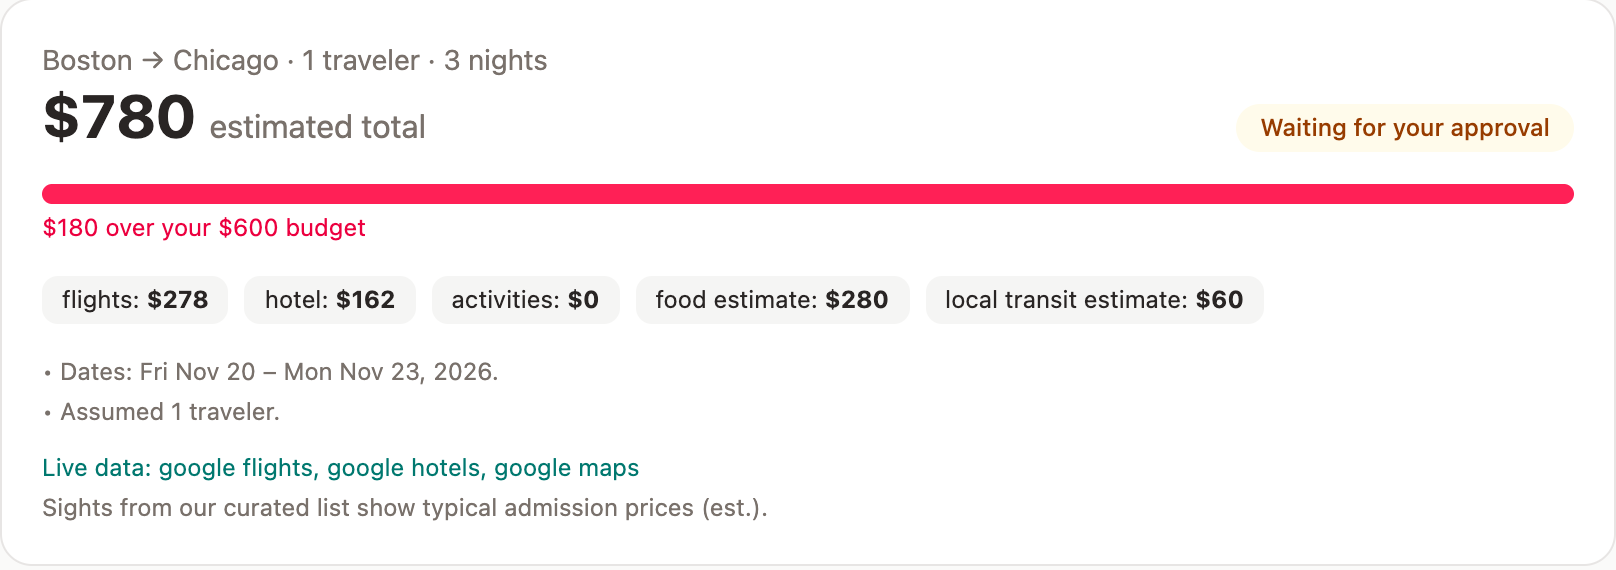
\includegraphics[width=\linewidth]{esc_budget.png}
      \figcaption{The plan in Alex's run: the budget bar turns red, and the plan waits for approval.}
    \end{column}
    \begin{column}{0.38\textwidth}
      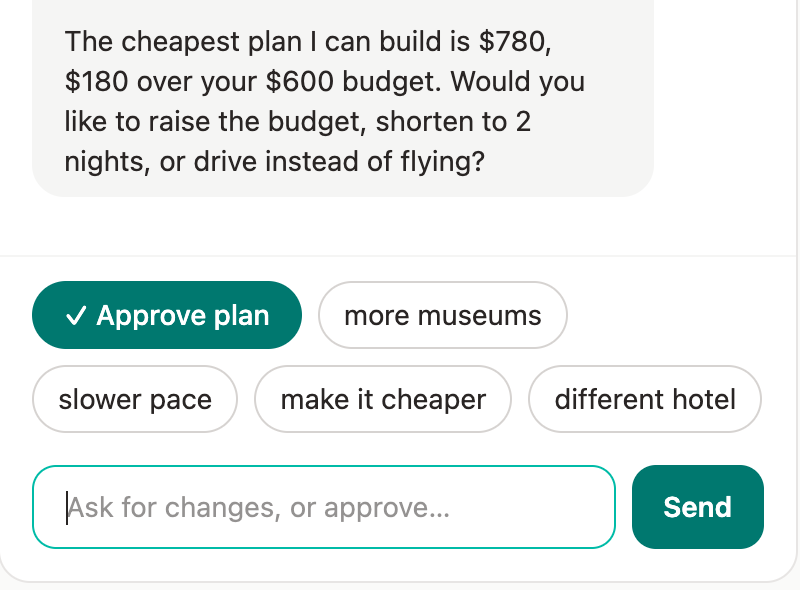
\includegraphics[width=\linewidth]{esc_question.png}
      \figcaption{The question in the chat, with buttons for a change or approval.}
    \end{column}
  \end{columns}
  \vspace{0.35cm}
  {\normalsize\bfseries Alex's call\par}
  \vspace{0.2cm}
  \option{raise the budget}\hspace{0.5em}\option{shorten to 2 nights}\hspace{0.5em}\option{drive instead of flying}\par
  \vfill
  \support{Alex picks one. The plan is \textbf{rebuilt and checked again}, then waits for Alex.}
  \vspace{0.05cm}
  \support{{\color{ok}\faCalendarCheck\ \textbf{Approve}} only exports a calendar file. Roameo never books or pays for anything.}
  \vspace{0.15cm}
  \note{
    \textbf{(36s, ends 3:47)} So Roameo stops and asks. The bar turns red: one hundred eighty
    dollars over your six hundred dollar budget. Would you like to raise the budget, shorten to
    two nights, or drive instead of flying? This is the moment that matters. The agents did the
    work, but the trade-off belongs to Alex. Alex picks one, the plan is rebuilt and checked
    again, and it waits. Nothing is final until Alex approves, and approving only exports a
    calendar file. Roameo never books or pays.
  }
\end{frame}

% ~~~~~~~~~~~~~~~~~~~~~~~~~~~~~~~~~~~~~~~~~~~~~~~~~~~~~~~~~~~~~~~~~~~~~~~~~~~~~~
% 7. ADAPTIVE AND VERSATILE (42 s)
\begin{frame}{Plans bend to feedback, weather and the season}
  \vspace{0.0cm}
  {\small Say it in plain words:\quad}\option{cheaper}\hspace{0.3em}\option{different hotel}\hspace{0.3em}\option{skip a place}\hspace{0.3em}\option{more museums}\hspace{0.3em}\option{slower pace}
  \vspace{0.35cm}
  \begin{columns}[T]
    \begin{column}{0.40\textwidth}
      
\includegraphics[width=\linewidth]{winter_ask.png}
      \vspace{0.1cm}
      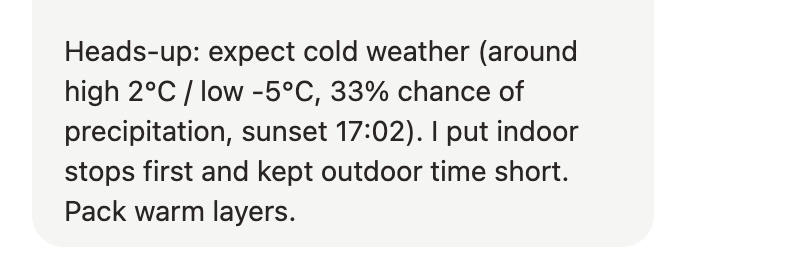
\includegraphics[width=\linewidth]{winter_warn.png}
      \figcaption{Michigan in December: it asks which city, then warns about the cold and puts indoor stops first.}
    \end{column}
    \begin{column}{0.58\textwidth}
      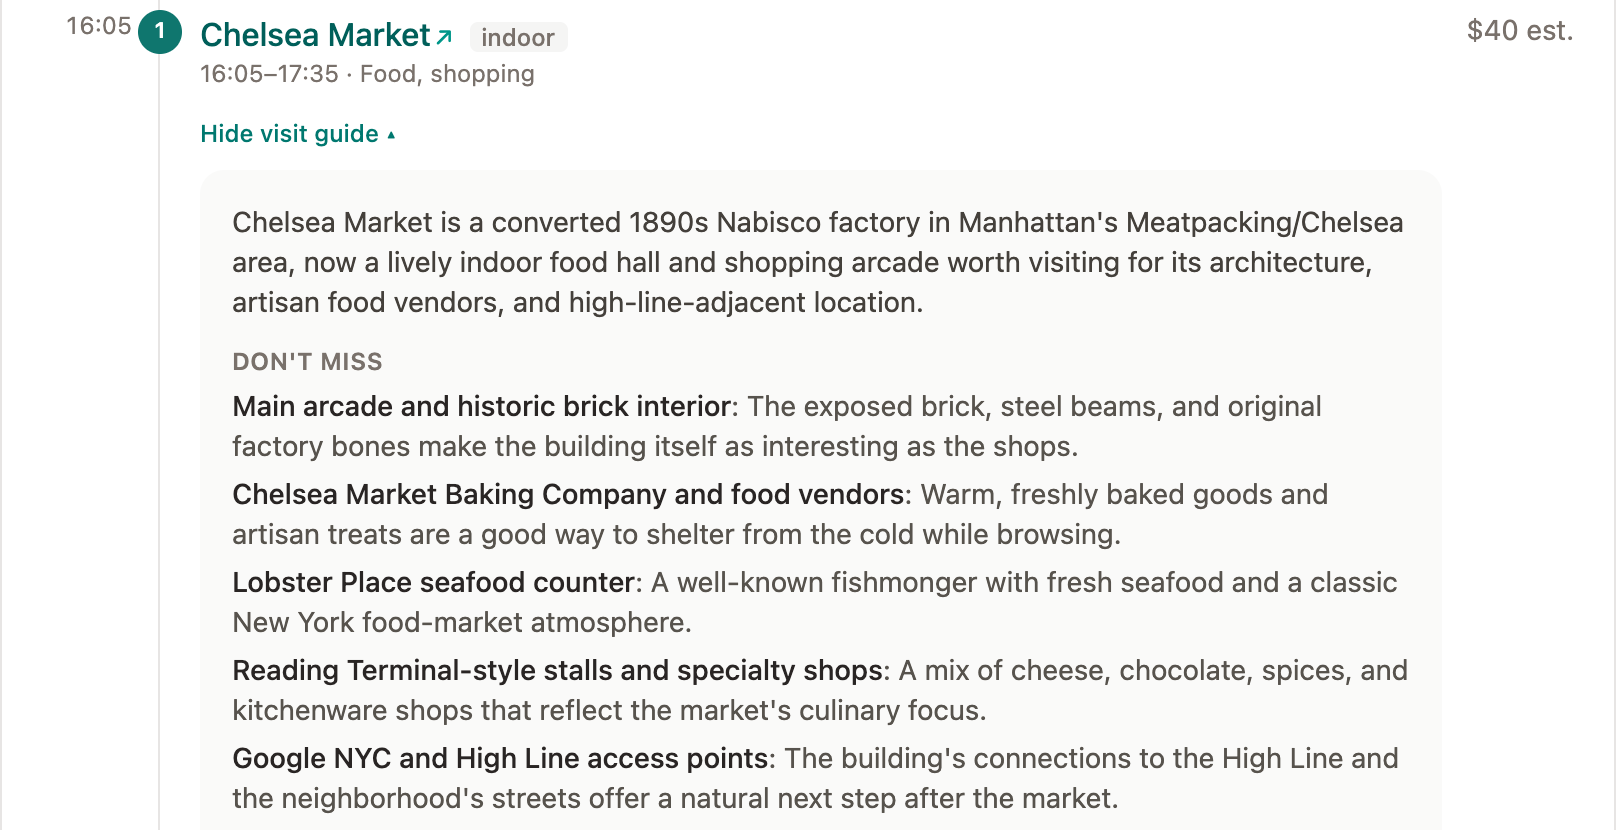
\includegraphics[width=\linewidth]{guide_top.png}
      \figcaption{A visit guide for one stop: what it is and what not to miss.}
    \end{column}
  \end{columns}
  \vfill
  \support{Each request is an \textbf{edit, not a restart}: the rest of the plan stays, and the reply lists what changed.}
  \vspace{0.15cm}
  \note{
    \textbf{(44s, ends 4:31)} Plans also bend. Alex can say cheaper, different hotel, skip a
    place, more museums or slower pace. Each request is an edit, not a restart, and the reply
    lists what changed. Weather and season count too. Here someone asks for Michigan in
    December. Michigan is a state, so it asks which city, then uses what those dates were like
    in past years, puts indoor stops first and says pack warm layers. And with the AI on, every
    stop gets a visit guide: what not to miss, and how to spend the time there. For museums,
    exhibitions come only from a real web search.
  }
\end{frame}

% ~~~~~~~~~~~~~~~~~~~~~~~~~~~~~~~~~~~~~~~~~~~~~~~~~~~~~~~~~~~~~~~~~~~~~~~~~~~~~~
% 8. RESULTS (56 s)
\begin{frame}{All 23 core tests pass in both modes, and in each of three AI runs}
  \vspace{0.0cm}
  \begin{center}
    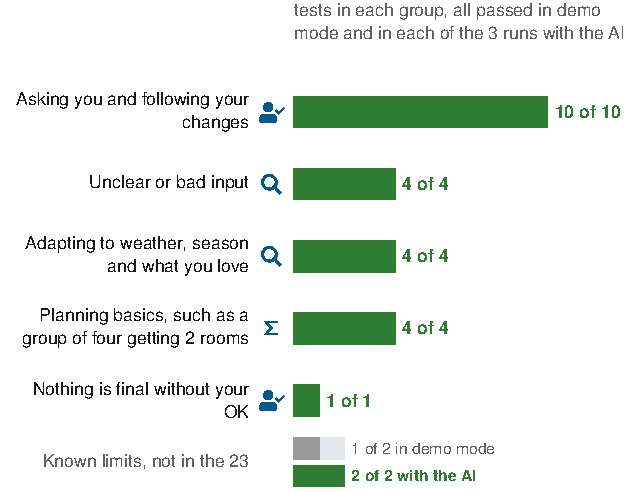
\includegraphics[height=6.25cm]{fig_results.pdf}
  \end{center}
  \vfill
  \support{A \textbf{test} is a scripted conversation with checks on the result, such as \emph{total within budget} or \emph{no flight search for a road trip}: 51 checks, all passed.}
  \vspace{0.05cm}
  \support{We wrote the tests ourselves, on sample prices. Demo mode follows fixed rules, so only the 3 AI runs speak to consistency.}
  \vspace{0.1cm}
  \note{
    \textbf{(54s, ends 5:25)} Does it work? We wrote twenty five test conversations. Each is a
    scripted chat followed by checks on the result, for example, the total is within budget, or
    there is no flight search for a road trip. Twenty three are core tests, and two are known
    limits that we report anyway. The core tests pass in demo mode, which follows fixed rules,
    and in AI mode, with Claude Haiku through OpenRouter. We ran AI mode three times, and every
    core test passed each time. Most tests are about asking you and taking feedback. But we
    wrote the tests, the tools used sample prices, and three runs is a small sample. Demo mode
    gives the same answer every time, so only the AI runs tell us about consistency.
  }
\end{frame}

% ~~~~~~~~~~~~~~~~~~~~~~~~~~~~~~~~~~~~~~~~~~~~~~~~~~~~~~~~~~~~~~~~~~~~~~~~~~~~~~
% 9. LIMITS (27 s)
\begin{frame}{What it cannot do yet}
  \vfill
  \begin{center}
    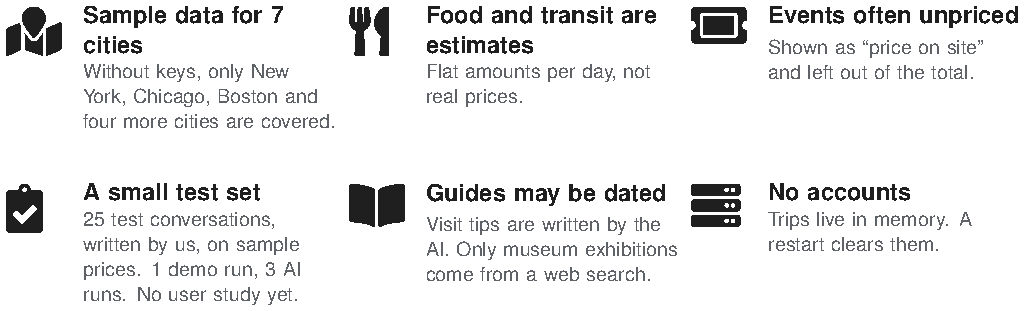
\includegraphics[width=\textwidth]{fig_limits.pdf}
  \end{center}
  \vfill
  \support{The tests do not judge how good a plan is, live prices, or the visit guides.}
  \vspace{0.2cm}
  \note{
    \textbf{(31s, ends 5:56)} What it cannot do yet. Without keys it covers seven cities. Food
    and local transit are flat daily estimates. Many events list no price, so they stay out of
    the total. Visit tips are written by the AI and may be out of date. Trips live in memory, so
    a restart clears them. And there was no user study. The tests do not judge how good a plan
    is, or live prices.
  }
\end{frame}

% ~~~~~~~~~~~~~~~~~~~~~~~~~~~~~~~~~~~~~~~~~~~~~~~~~~~~~~~~~~~~~~~~~~~~~~~~~~~~~~
% 10. DEPLOY AND WHO IT HELPS (38 s)
\begin{frame}{One URL to deploy, three minutes to try without keys}
  \vfill
  \begin{center}
    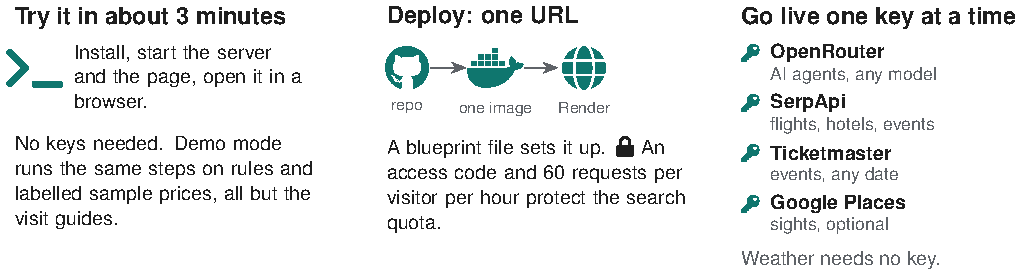
\includegraphics[width=\textwidth]{fig_deploy.pdf}
  \end{center}
  \vfill
  \support{Built for \textbf{students and budget travellers} on short trips, and for small groups who split the cost.}
  \vspace{0.05cm}
  \support{The free Render plan sleeps after 15 idle minutes, so open it a minute before you need it.}
  \vspace{0.2cm}
  \note{
    \textbf{(38s, ends 6:34)} It is easy to run. Without any keys, it starts on a laptop in
    about three minutes. To share it, one Docker image and a blueprint file put it on Render as
    one web address. An access code and sixty requests per visitor per hour protect the search
    quota. The free plan sleeps after fifteen idle minutes, so open it a minute early. Then add
    keys one at a time, with any OpenRouter model for the agents. It is built for students and
    budget travellers on short trips.
  }
\end{frame}

% ~~~~~~~~~~~~~~~~~~~~~~~~~~~~~~~~~~~~~~~~~~~~~~~~~~~~~~~~~~~~~~~~~~~~~~~~~~~~~~
% 11. CLOSE (13 s)
\begin{frame}{Alex still makes the call on the \$600}
  \budget{ink}{\$600, Alex's call}
  \vspace{0.9cm}
  \begin{columns}[T]
    \begin{column}{0.60\textwidth}
      {\Large Roameo's agents do the \textbf{research} and the \textbf{arithmetic}. When the money does not work out, they \textbf{stop and ask}, instead of quietly going over.\par}
      \vspace{0.8cm}
      \option{raise the budget}\hspace{0.4em}\option{shorten to 2 nights}\hspace{0.4em}\option{drive instead}\par
      \vspace{1.0cm}
      {\Large\bfseries Thank you\par}
      \vspace{0.15cm}
      {\normalsize Zhen Lu \quad Noctis Zhang\par}
    \end{column}
    \begin{column}{0.38\textwidth}
      
\begin{tikzpicture}[x=1cm, y=1cm]
        \node[anchor=north west, inner sep=0pt] at (0,0) {\qrcode[height=2.9cm]{https://roameo-l13h.onrender.com/}};
        \node[anchor=north west, inner sep=0pt, align=left, font=\small] at (3.15,-0.1) {\textbf{Try it}\\live demo};
        \node[anchor=north west, inner sep=0pt] at (0,-3.35) {\qrcode[height=2.9cm]{https://github.com/TinyZhen/Travel_Agent}};
        \node[anchor=north west, inner sep=0pt, align=left, font=\small] at (3.15,-3.45) {\textbf{Code}\\GitHub};
      \end{tikzpicture}
    \end{column}
  \end{columns}
  \note{
    \textbf{(13s, ends 6:47)} Back to Alex. Roameo did the research and the math, and showed the
    gap honestly. The six hundred dollars stays Alex's call. Scan the code to try it. Thank you.
  }
\end{frame}

% ~~~~~~~~~~~~~~~~~~~~~~~~~~~~~~~~~~~~~~~~~~~~~~~~~~~~~~~~~~~~~~~~~~~~~~~~~~~~~~
% BACKUP SLIDES (not timed)
\appendix
\begin{frame}{Backup: the critic's repairs, in a fixed order}
  \vspace{0.3cm}
  \begin{center}
    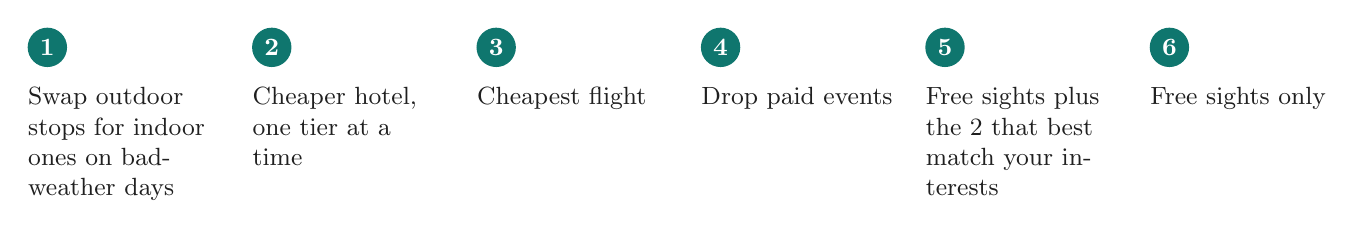
\begin{tikzpicture}[x=1cm, y=1cm, font=\small,
      st/.style={anchor=north west, text width=2.45cm, align=left, inner sep=0pt, text=ink},
      no/.style={circle, fill=primary, text=white, font=\small\bfseries, inner sep=1.6pt, minimum size=5mm}]
      \foreach \i/\x/\t in {1/0/{Swap outdoor stops for indoor ones on bad-weather days}, 2/2.85/{Cheaper hotel, one tier at a time}, 3/5.7/{Cheapest flight}, 4/8.55/{Drop paid events}, 5/11.4/{Free sights plus the 2 that best match your interests}, 6/14.25/{Free sights only}} {
        \node[no] at (\x+0.25,0.3) {\i};
        \node[st] at (\x,-0.2) {\t};
      }
    \end{tikzpicture}
  \end{center}
  \vspace{0.6cm}
  \support{The critic applies one repair, the composer rebuilds and prices the plan, and the critic checks again, at most five times. If the plan is still over budget, the person decides, so the last repair may never run. The weather swap runs first whenever a rainy day has outdoor stops. In Alex's run that happened only after the sights changed, so it came last. Budget repairs run only while the plan is over budget.}
  \vspace{0.3cm}
  \support{Escalation also covers no flight, no hotel, light days and cold weather. In the AI mode, a failed model call falls back to the rule path, so some AI-mode passes may use rules.}
  \note{Backup only. Source: the critic agent's repair order and the coordinator's limit of five repairs.}
\end{frame}

\begin{frame}{Backup: what the 25 test conversations check}
  \vspace{0.1cm}
  {\footnotesize\renewcommand{\arraystretch}{1.35}
  \begin{tabularx}{\textwidth}{@{}>{\raggedright\arraybackslash}p{3.7cm}>{\raggedright\arraybackslash}X@{}}
    \textbf{Asking you and feedback (10)} & Missing date, missing destination and missing origin are asked, never assumed. An impossible budget is escalated. Raising the budget makes the plan fit. ``Cheaper'' really lowers the price, ``different hotel'' changes it, a named place is skipped. ``More museums'' revises, ``slower pace'' lightens the days. \\
    \textbf{Bad input, no guessing (4)} & Unknown city, a past date, vague feedback, a state instead of a city. \\
    \textbf{Weather, season, interests (4)} & Rainy days start indoors, winter days keep outdoor time short, a river cruise is not scheduled out of season, cutting cost keeps a museum for a museum lover. \\
    \textbf{Core planning (4)} & A complete request gives a priced plan within budget, driving skips flights and adds gas and parking, a local day trip has no flight or hotel, a family of four gets two rooms. \\
    \textbf{Safety (1)} & Nothing is approved without an explicit approval. \\
    \textbf{Known limits (2)} & A city outside the demo data is asked about. A complex date phrase: demo mode asks for a date instead, AI mode resolves it. \\
  \end{tabularx}}
  \vspace{0.2cm}
  \figcaption{From the results files in the repository: demo mode with 1 run, AI mode with 3 runs per test.}
  \note{Backup only.}
\end{frame}

\end{document}
